\documentclass{scrartcl}
\usepackage[utf8]{inputenc}
\usepackage[ngerman]{babel}
\usepackage{amsmath}
\usepackage{graphicx}

\usepackage{caption, booktabs}


\usepackage{fixltx2e}
\usepackage[aux]{rerunfilecheck}
\usepackage{polyglossia}
\setmainlanguage{german}
\usepackage{ngerman}%ae usw


\usepackage{amsmath}

\usepackage{fontspec}

\usepackage[
  locale=DE,
  separate-uncertainty=true,
  per-mode=symbol-or-fraction,
]{siunitx}

\usepackage{float}
\usepackage[section, below]{placeins}

\usepackage[unicode]{hyperref}
\usepackage{bookmark}

\floatplacement{figure}{htbp}
\floatplacement{table}{htbp}

\title{V51 Schaltungen mit Operationsverstärkern}
\author{Ismael Abu-Nada \footnote{ismael.abunada@tu-dortmund.de}\and Burak Kabakci\footnote{burak.kabakci@tu-dortmund.de}}
\date{18. April 2018}

\makeatletter
\def\@fnsymbol#1{\ensuremath{\ifcase#1\or *\or ** \else\@ctrerr\fi}}
\makeatother
\begin{document}
	\maketitle
	\begin{center}
		TU Dortmund Physikalisches Fortgeschrittenen Praktikum
	\end{center}
	\thispagestyle{empty}
	\newpage
	\tableofcontents


\newpage

\section{Einleitung }

Operationsverstärker gehören zu den wichtigsten integrierten Schaltungen der Elektrotechnik. In diesem Versuch werden einige grundlegende Schaltungen aufgebaut und untersucht.

\section{Theorie}

Der Operationsverstärker ist ein gleichstromgekoppelter Differenzverstärker, der einen nicht-invertierenden Eingang (Kennzeichnung durch ein + im Schaltsymbol) und einen invertierenden Eingang (Kennzeichnung durch ein - im Schaltsymbol), sowie einen Ausgang dessen Spannung $U_A$ proportional zur Spannungsdifferenz an den beiden Eingängen ist, besitzt (siehe Abb. \ref{schalt}).
$U_A$ ist gegeben durch
\begin{align}
U_\mathrm{A} = V(U_\mathrm{p}-U_\mathrm{N})
\end{align}
Der Faktor $V$ wird als die Leerlaufverstärkung bezeichnet.
%$V$ ist dabei die frequenzunabhängige Leerlaufverstärkung die nur bei hohen Frequenzen Frequenzabhängkeit aufweist.
Des Weiteren kann die Ausgangspannung kann nur im Bereich $-U_\mathrm{B} < U_\mathrm{A} < U_\mathrm{B}$ der Betriebsspannung $U_\mathrm{B}$ variieren, wobei ein linearer Zusammenhang vorliegt (Aussteuerungsbereich), danach bleibt $U_A$ gesättigt auf der positiven oder negativen Betriebsspannung.
\iffalse
\begin{figure}[H]
  \centering
  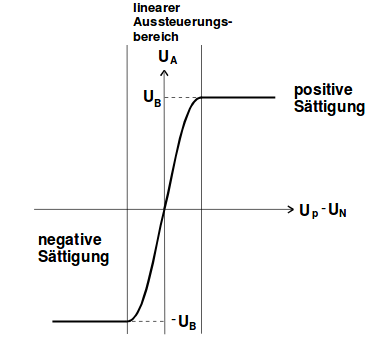
\includegraphics[width=4cm]{spannungsverlauf.jpg}
  \caption{Ausgangsspannung $U_A$ als Funktion der Spannungsdifferenz der Eingangsspannungen beim Operationsverstärker [1]}
  \label{dreck}
\end{figure}
\fi

\begin{figure}[!h]
\centering
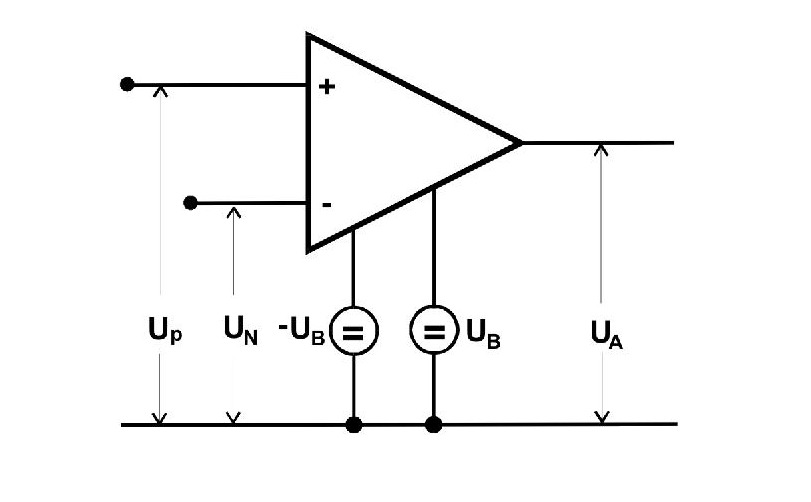
\includegraphics[width=0.6\textwidth]{schaltsymbol}
\caption{Schaltsymbol eines Operationsverstärkers. [1]}
\label{schalt}
\end{figure}

\subsection{Kenngrößen des realen und idealen Operationsverstärkers}
Es wird grundsätzlichen zwischen einem idealen Operationsverstärker und realen Operationsverstärker unterschieden. Der ideale Operationsverstärker ist eine vereinfachte Annahme des realen Operationsverstärkers und wird eingeführt, um die Berechnung von Schaltungen mit Operationsverstärkern zu vereinfachen. Wichtige Kenngrößen eines realen Operationsverstärkers sind neben der Leerlaufverstärkung die Eingangswiderstände $r_\mathrm{e_\mathrm{p}}$ und $r_\mathrm{e_\mathrm{n}}$ und der Ausgangswiderstand $r_\mathrm{a}$. Da bei einem realen Operationsverstärker die Werte für die Leerlaufverstärkung und die Eingangswiderstände sehr große Werte und für den Ausgangswiderstand ein sehr kleiner Wert erreicht wird, sind die Kenngrößen bei einem idealen Operationsverstärker wie folgt definiert:
\begin{align*}
V_\mathrm{id} &= \infty& ,
r_\mathrm{e_\mathrm{id}} &= \infty& ,
r_\mathrm{a_\mathrm{id}} &= 0
\end{align*}
Für eine korrekte Berechnung eines realen Verstärkers müssen noch weitere Kenngrößen eingeführt werden, die beim idealen Operationsverstärker den Wert 0 oder Unendlich haben: Die Gleichtaktverstärkung, der Eingangsruhestrom, der Offsetstrom/die Offsetspannung, der Differenz-/Gleichtakteingangswiederstand.
Diese Kenngrößen dienen lediglich dazu die Schaltung in Feinheiten korrekt beschreiben zu können und können laut Aufgabenstellung vernachlässigt werden.

\subsection{Schaltungen}
\subsubsection{Der gegengekoppelte invertierende Linearverstärker}
Ein Operationsverstärker besitzt aufgrund seiner hohen Leerlaufverstärkung  nur einen schmalen Aussteuerungsbereich. Daher ist er ohne einen Gegenkopplungszweig in der Praxis als Linearverstärker unbrauchbar. Beim gegengekoppelten invertierenden Verstärker wird eine Rückkopplung auf den invertierenden Eingang gelegt. Dies hat zur Folge, dass die Gesamtverstärkung gegenüber der Leerlaufverstärkung abnimmt, es kommt zur Streckung des Aussteuerungsbereiches.
Da wie beim idealen Operationsverstärker für die Berechnungen von $V = \infty, r_e=\infty$ ausgegangen wird, ist

  \begin{align*}
    U_N &= -\frac{U_A}{V} = 0,
    \text{und},
    I_N = \frac{U_N}{r_e} = 0,
  \end{align*}
 Somit gilt für den Knotenpunkt A in Abb. 2 nach der Kirchhoff'schen Knotenregel:
%Aufgrund der sehr hohen Leerlaufverstärkung  ist die Spannung $U_N$ gleich null. Damit gilt nach der Kirchhoffschen Knotenregel für den Knotenpunkt A in Abb. 2
\begin{equation*}
  I_A=I_R \iff \frac{U_1}{R_1}=-\frac{U_A}{R_N} \iff U_A=-\frac{R_N}{R_1}U_1
\end{equation*}
Daher ist die Verstärkung/der Verstärkungsfaktor $V'$:
\begin{equation}
  %V'=\frac{R_N}{R_1}=\frac{U_A}{U_1}
\end{equation}

\iffalse
 \begin{align}
\frac{U_1}{R_1} + \frac{U_\text{A}}{R_\text{N}} = 0\;\;
\end{align}
Die als Verhältnis von Ausgangsspannung zu Eingansspannung definierte Verstärkung $V'$ lautet somit:
\begin{align}
V' := \frac{U_\mathrm{A}}{U_\mathrm{E}} = - \frac{R_\mathrm{N}}{R_1}
\end{align}
Im weiterem wird nur der Einfluss einer endlichen Leerlaufverstärkung $V$ auf den Verstärkungsfaktor $V'$ betrachtet, daher gilt:
\begin{align}
U_\text{N} = -\frac{U_\text{A}}{V}
\label{spannung}
\end{align}
Mit $I_N = 0$ folgt für den unbelasteten Spannungsteiler am Knotenpunkt A
\begin{align}
\frac{U_\text{N}-U_1}{U_\text{A}-U_1} = \frac{R_1}{R_1 + R_\text{N}}\;\;.
\label{spannungsteiler}
\end{align}
Aus (4) und (5) folgt nach Elimination von $U_N$ das Verhältnis $V'$
\begin{align}
\frac{1}{V'} = \frac{1}{V} + \frac{R_1}{R_\text{N}} \left( 1 + \frac{1}{V} \right) \approx \frac{1}{V} + \frac{R_1}{R_\mathrm{N}}.
\label{eq:leerlauf}
\end{align}
\fi %alles auskommentiert

\begin{figure}[!h]
\centering
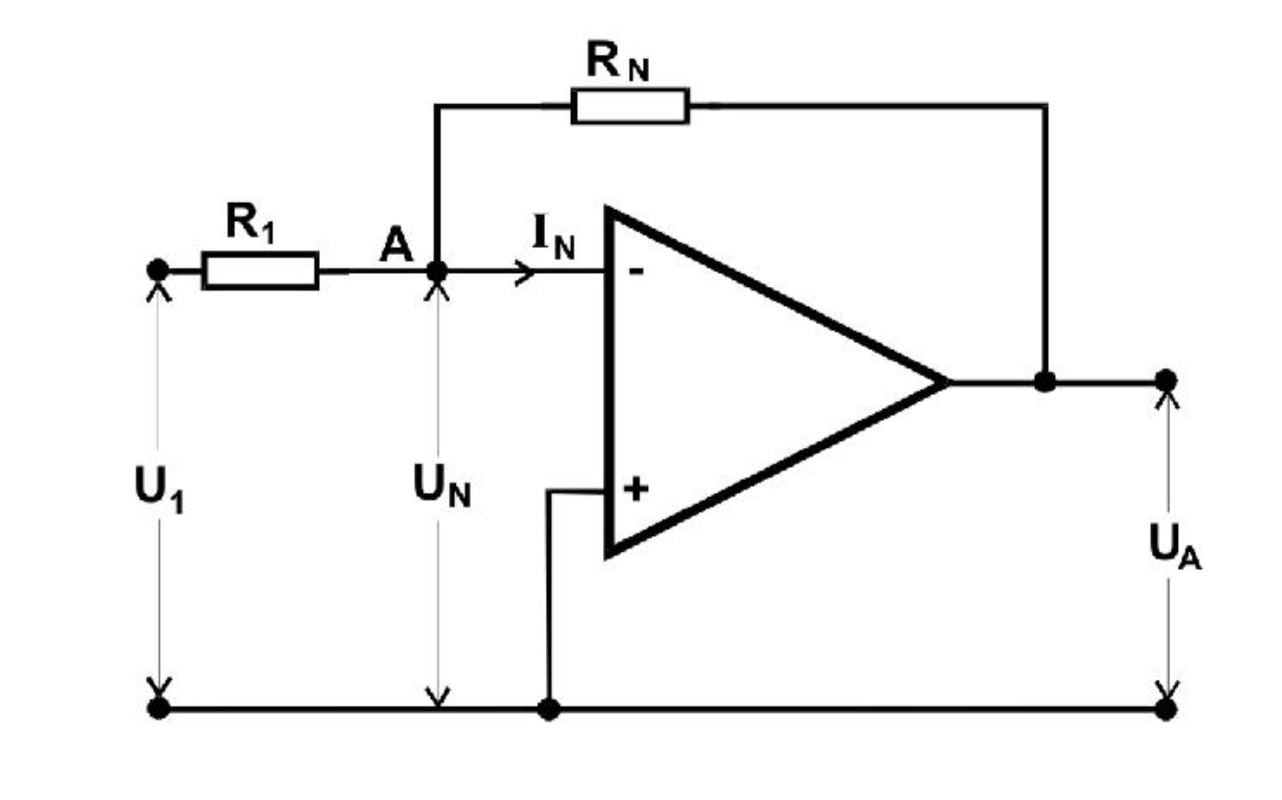
\includegraphics[width=0.6\textwidth]{invertierender}
\caption{Schaltplan eines invertierenden Verstärkers. [1]}
\label{verstaerker}
\end{figure}
Wird hingegen von einem realen Operationsverstärker aussgegangen, aber nur der Effekt der endlichen Leerlaufverstärkung $V$ auf den Verstärkungsfaktor $V'$ berücksichtigt, wird die Beziehung
\begin{equation}
  \frac{1}{V'} = \frac{1}{V} + \frac{R_1}{R_\mathrm{N}} \left(1+\frac{1}{V}\right)
  \iff V = \frac{1 + \frac{R_1}{R_\text{N}}}{\frac{1}{V'}-\frac{R_1}{R_\text{N}}}
  \label{lappen1}
\end{equation}
Damit lässt sich ein endlicher Verstärkungsfaktor $V$ berechnen.
Bei einer starken Gegenkopplung, also geringem Verstärkungsgrad wird die ideale Beziehung herhalten, bei die Verstärkung $V'$ quasi unabhängig von der Leerlaufverstärkung $V$, welche temperaturabhängig ist.
Eine starke Gegenkopplung sorgt deshalb für Stabilität der Verstärkungsschaltung.
%Durch eine starke Gegenkopplung entwirft man einen Verstärker mit geringem Verstärkungsgrad. Daher hängt seine Verstärkung vom Teilerverhältnis der beiden Widerstände ab. Demzufolge haben Schwankungen von $V$ durch Temperaturänderungen oder ähnliche Effekte also (fast) keinen Einfluss auf $V'$, das heißt die Stabilität der Verstärkerschaltung wird durch eine Gegenkopplung erhöht.

\subsubsection{Der Umkehr-Integrator}
Das Eingangssignal wird durch den Einbau einer Kapazität $C$ in den Rückkopplungszweig (siehe Abb. 3) integriert. Man berücksichtigt
\begin{align}
\int I_\text{C}\,\text{dt} = CU_\text{A}
\end{align}
 und wendet die Knotenregel am Verzweigungspunkt A, um auf die Beziehung zu kommen
\begin{align*}
U_\mathrm{A} = - \frac{1}{RC} \int U_1 (t) \mathrm{d}t \;\;.
\end{align*}
Hier ist $U_1$ eine Sinusspannung, also $U_1 = U_0 \sin (\omega t)$ und es folgt
\begin{align}
U_\mathrm{A} = \frac{U_0}{\omega RC} \cos (\omega t)\;.
\end{align}
Bei einer Sinusspannung sind Ausgangsspannung und Frequenz umgekehrt proportional zueinander.
\begin{figure}[!h]
\centering
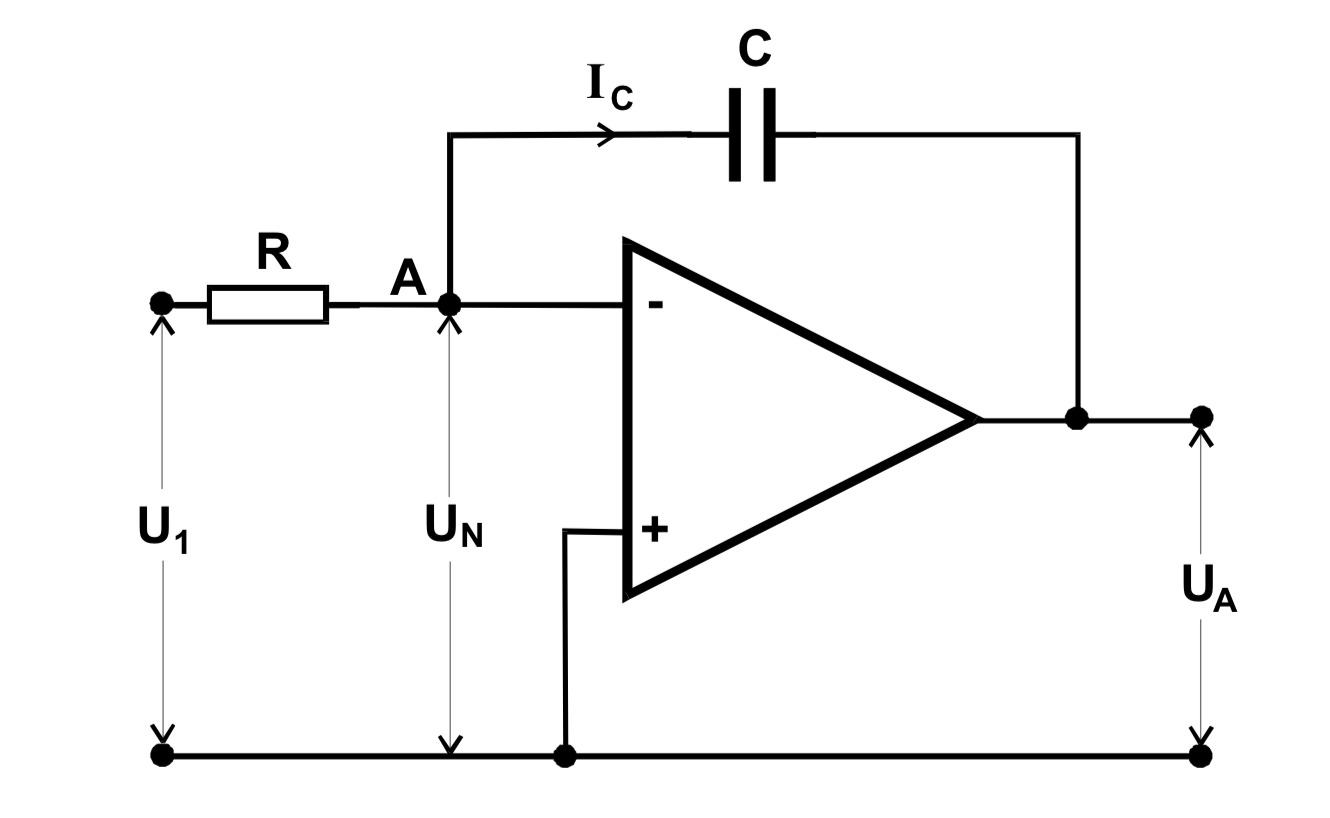
\includegraphics[width=0.6\textwidth]{integrator}
\caption{Schaltplan einer integrierenden Schaltung. [1]}
\label{integrator}
\end{figure}

\newpage

\subsubsection{Der Differentiator}
Beim Differentiator wird die Kapazität mit dem Widerstand verstauscht (siehe Abbildung 4). Dadurch erhält man als Ergebnis die Ausgangsspannung $U_A$ die proportional zum Differentialquotienten der Eingangsspannung ist:
\begin{align*}
U_\mathrm{A} = - RC \frac{\mathrm{d}U_1}{\mathrm{d}t} \;\;.
\end{align*}
Dabei ist $U_1$ wie bei 2.2.2 eine Sinusspannung, also $U_1 = U_0 \sin (\omega t)$ und es folgt
\begin{align}
U_\mathrm{A} = - \omega RC U_0 \cos (\omega t)\;\;,
\label{timbugtu}
\end{align}
also eine direkte Proportionalität zwischen der Amplitude der Ausgangsspannung zur Frequenz.
\begin{figure}[!h]
\centering
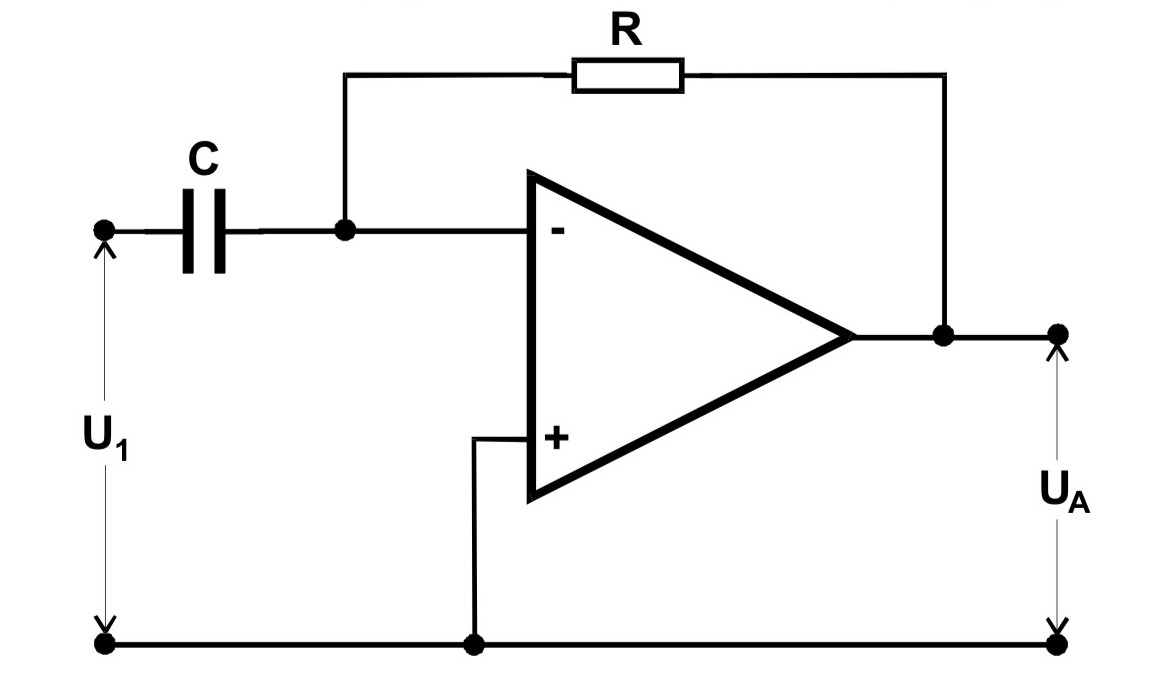
\includegraphics[width=0.6\textwidth]{differentiator}
\caption{Schaltplan einer Differentiator-Schaltung. [1]}
\label{differentiator}
\end{figure}

\subsubsection{Der Schmitt- Trigger}
Beim Schmitt- Trigger wird ein Teil der Ausgangsspannung auf den nicht-invertierenden Eingang rückgekoppelt (siehe Abbildung 5), dadurch wird die Ausgangspannung $U_\text{A}$ laufend erhöt bzw. erniedriegt, bis sie den Sättigungswert/die Betriebsspannung $\pm U_\text{B}$ erreicht.
Dabei springt die Ausgangsspannung auf den postiven Sättigungswert/die positive Betriebsspannung $+U_B$ sobald die Speisespannung $U_1$ die positive Schwellspannung
\begin{equation}
  \frac{R_1}{R_\text{p}}U_B
\end{equation}
überschritten hat und auf den negativen Sättigungswert $-U_B$ sobald die Speisespannung den Wert
\begin{equation}
  -\frac{R_1}{R_\text{p}}U_B
\end{equation}
unterschritten hat, da $U_p$ (Abb. 5) bei diesen Werten ihr Vorzeichen wechselt.
%Dieser Prozess beginnt allerdings erst, sobald der Betrag Speisespannung $U_1$ die Schwelle

%wechselt die Ausgangsspannung ihr Vorzeichen. Wird die Schwelle überschritten springt die Ausgangsspannung $U_A$ auf den Wert $+U_B$, wird sie unterschritten springt sie auf den Wert $-U_B$.
\begin{figure}[!h]
\centering
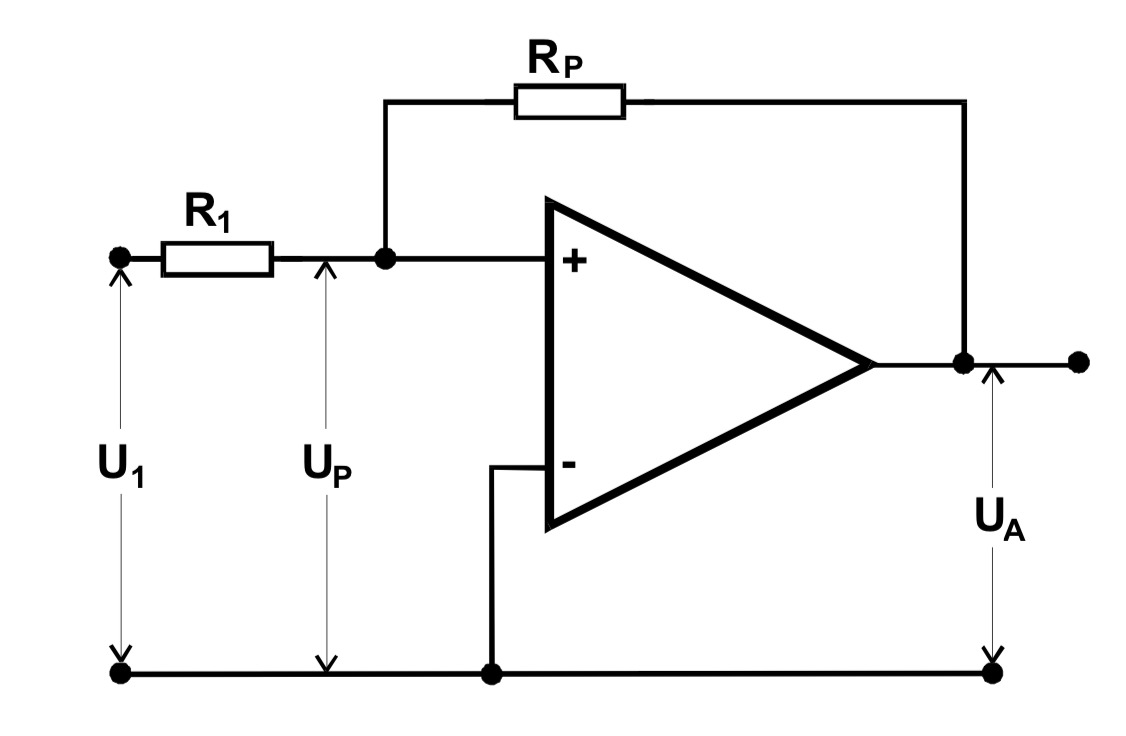
\includegraphics[width=0.6\textwidth]{schmitt}
\caption{Schaltplan eines Schmitt-Triggers. [1]}
\label{schmitt}
\end{figure}
In Abb. \ref{hyst} ist die Hysterese des Schmitt-Triggers qualitativ dargestellt.
\begin{figure}[!h]
\centering
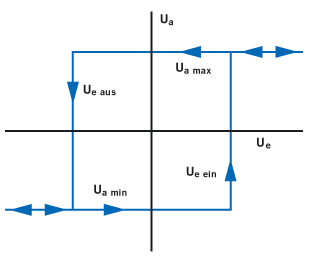
\includegraphics[width=0.6\textwidth]{hyst.png}
\caption{Hysterese des Schmitt-Triggers [2]}
\label{hyst}
\end{figure}
\FloatBarrier

\subsubsection{Die Nachbildung einer linearen Schwingungsdifferentialgleichung mit Operationsverstärkern}
Mit der Schaltung (siehe Abbildung \ref{harm}), können exponentiell mit der Zeit zu- oder abnehmende Sinusschwingungen erzeugt werden. Die Schaltung besteht aus zwei Integratoren und einem Invertierer. Die Schaltung wird durch die Differentialgleichung
\begin{align}
\frac{\mathrm{d}^2 U_\mathrm{A}}{\mathrm{d}t^2} - \frac{\eta}{10 RC}\frac{\mathrm{d}U_\mathrm{A}}{\mathrm{d}t} + \frac{1}{(RC)^2} U_\mathrm{A} = 0
\end{align}
beschreiben.  Die Lösung dieser Differentialgleichung ist durch
\begin{align}
U_\mathrm{A}(t) = U_0 \exp \left(\frac{t}{\tau} \right) \sin \left( 2 \pi \frac{t}{T} \right)
\end{align}
mit der Abklingdauer
\begin{align}
    \tau := \frac{20RC}{|\eta|}
    \label{schwingung:tau}
\end{align}
gegeben.
$\tau$ ist die Zeit für Abnahme/Zunahme der Amplitude auf den e-ten Teil/das e-fache ihres Ausgangswertes, für $\eta>0$ nimmt die Amplitude zu, für $\eta<0$ nimmt sie ab.
% Die Konstante $\eta$ sagt etwas über das Verhalten der Amlitude aus und wird durch ein Potentiometer eingestellt. Bei $\eta =1$ wächst die Amplitude nach der Zeit $20RC$ auf das $e$-Fache, bei $\eta =-1$ sinkt die Amplitude auf den $e$-tel Teil und bei $\eta$ =0 ist die Amplitude konstant. Die Wahl von $\eta$ bestimmt also, ob die Schwingung exponentiell ansteigend oder abfallend ist.
\begin{figure}[!h]
%\label{harm}
\centering
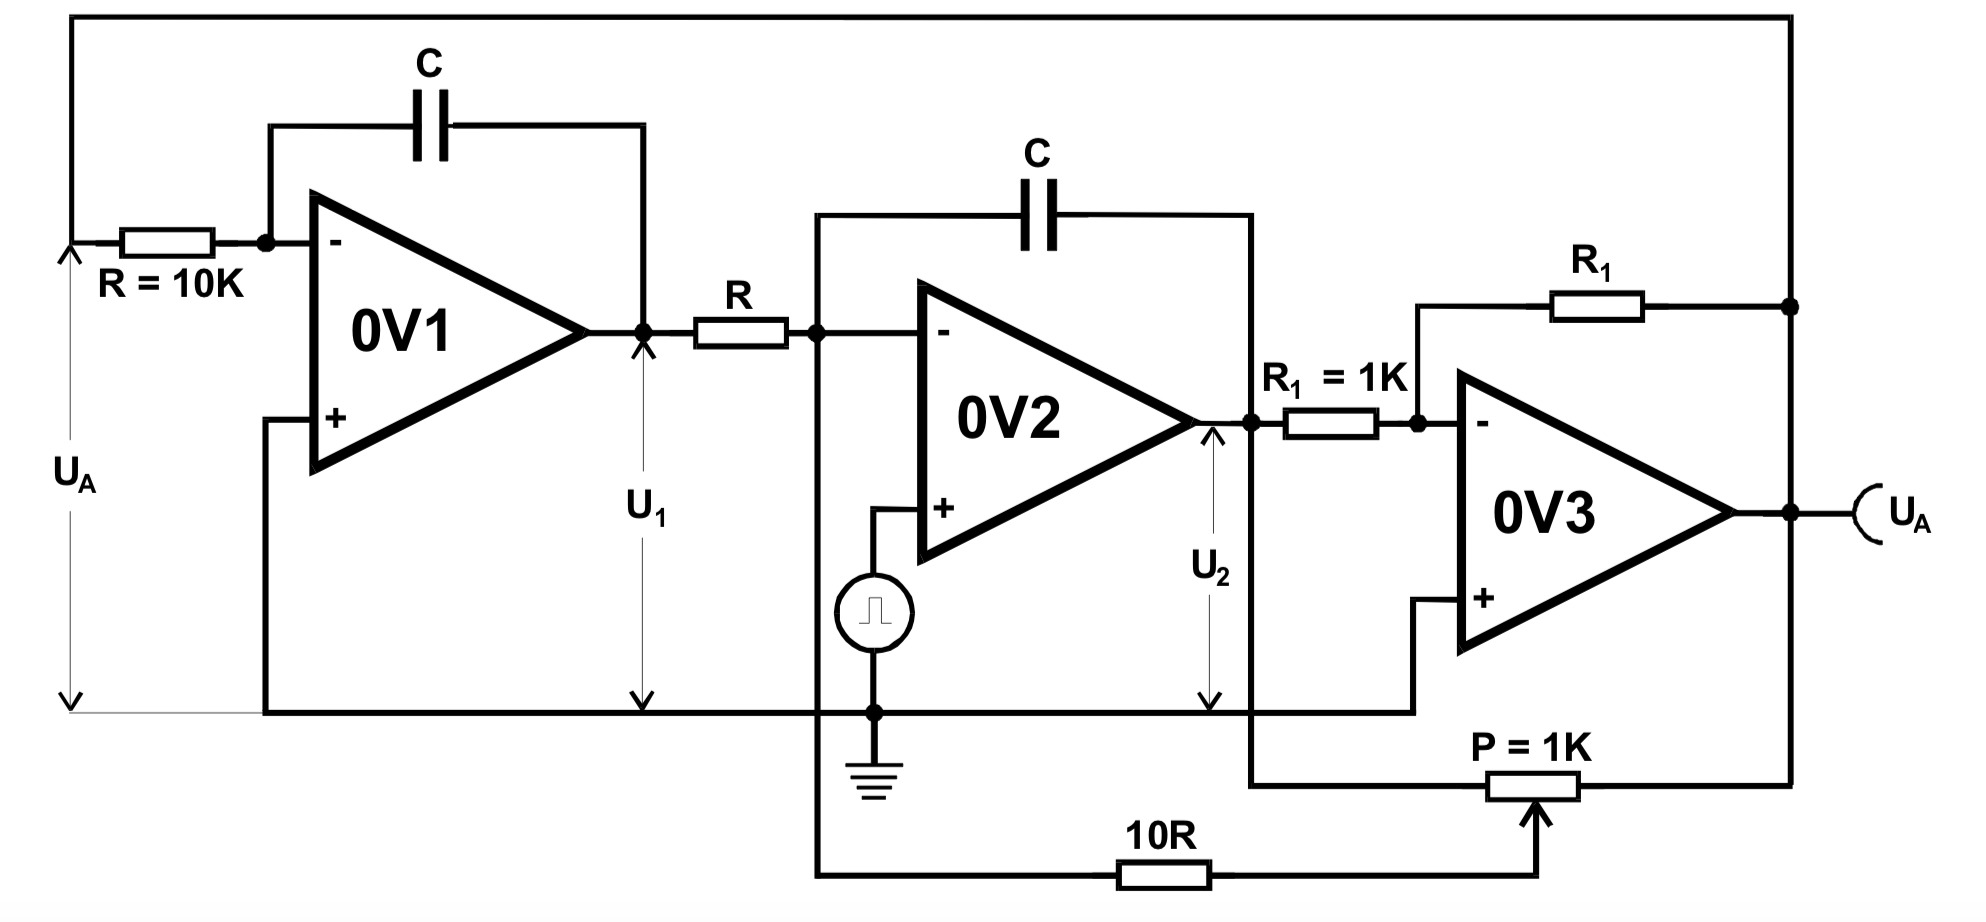
\includegraphics[width=0.7\textwidth]{gedschwingung}
\caption{Schaltplan zur Erzeugng einer gedämpften harmonischen Schwingung. [1]}
\label{harm}
\end{figure}

\section{Versuchsdurchführung}
\label{sec:Durchführung}
Bei der Versuchsdurchführung werden die Schaltungen des vorherigen Kapitels aufgebaut und untersucht:
\begin{itemize}
\item Beim gegengekoppelten invertierenden Linearverstärker (Abbildung 2) wird für vier verschiedene Verstärkungsgerade die Frequenzabhängigkeit untersucht.
\item Beim Umkehrintegrator und Umkehr-Differentiator (Abbildung 3 und 4) wird über ein Signalgenerator das Eingangsignal in Sinus-, Rechteck und Dreiecksspannung geändert und das Ergebnis wird an einem Oszilloskop kontrolliert. Wie beim gegengekoppelten invertierenden Linearverstärker wird auch hier die Frequenzabhängigkeit der Ausgangsspannung untersucht.
Dies wird für zwei verschiedene Paare der Widerstände gemacht.
\item Beim Schmitt-Trigger (Abbildung 5) wird der Wert bei der die Ausgangsspannung ihr Vorzeichen wechselt ermittelt, indem auf ein Oszilloskop das Schalterverhalten beobachtet wird.
\item Im letzten Versuchsteil wird eine gedämpfte und eine ungedämpfte Schwingung erzeugt und am Oszilloskop untersucht.
\end{itemize}



\section{Auswertung}

\subsection{Fehlerrechnung}
Zur Fehlerrechnung werden folgende Formeln verwendet.
Der Mittelwert:
\begin{align}
\bar{x} = \frac{1}{N} \sum_{i=1}^N x_i
\end{align}
Abweichung vom Mittelwert (Varianz):
\begin{align}
s_x^2 = \frac{1}{N(N-1)} \sum_{i=1}^N (x_i - \bar{x})^2
\end{align}
Fehlerfortpflanzung nach Gauß:
\begin{align}
\Delta_y = \sqrt{\sum_{i=1}^N \left(\frac{\partial y}{\partial x_i}\right)^2 \Delta x_i^2}
\end{align}

\subsection{Frequenzgänge des Linearverstärkers}
Es wurden vier Frequenzgänge für vier verschiedene Gegenkopplungen gemessen.  Die gemessenen Werte sind in den Tabellen 2-5 zu sehen. Die Fits wurden mit Gnuplot erstellt. Die Ausgleichsgeraden wurden mit Hilfe der Gleichung:
 \begin{align}
 f( \nu)=\alpha \cdot \nu ^\beta
 \end{align}
 erstellt.
Für die abfallenden Ausgleichsfunktionen der Frequenzgänge 1-4 ergab sich somit:
  \begin{align}
f_1(\nu)&=(10,80\pm0,78)\cdot \left(\frac{\nu}{\text{kHz}}\right)^{-0,18\pm0,03}\\
f_2(\nu)&=(3,14\pm0,16)\cdot \left(\frac{\nu}{\text{kHz}}\right)^{-0,06\pm0,01}\\
f_3(\nu)&=(56,80\pm4,80)\cdot \left(\frac{\nu}{\text{kHz}}\right)^{-0,30\pm0,05}\\
f_4(\nu)&=(33,85\pm2,67\cdot)\left(\frac{\nu}{\text{kHz}}\right)^{-0,27\pm 0,04}
 \end{align}
Das heißt, im doppelt-logarithmischen Diagramm ergeben sich Geraden mit der Steigung:
\begin{align}
  m_1=-0,18\pm0,03\\
  m_2=-0,06\pm0,01\\
  m_3=-0,30\pm0,05\\
  m_4=-0,27\pm0,04
\end{align}
Mit Hilfe des Mittelwerts der Verstärkung  $V′$ für annähernd konstante Werte, wird die Grenzfrequenz bestimmt.
Die Genzfrequenz wird bestimmt indem der Schnittpunkt der konstanten Geraden $\frac{\bar{V}'}{\sqrt{2}}$ mit der jeweiligen Ausgleichsfunktion  $f_i(\nu)$ bestimmt wird und dann der x-Achsenabschnitt abgelesen wird. Aus den zuvor berechneten Werten lässt sich das Verstärkungs-Bandbreite-Produkt durch die Formel

   \begin{align}
   \nu'_g \bar{V}' = const
 \end{align}
 überprüften.
Die Ergebnisse aller Berechnungen sind in Tabelle 1 aufgeführt.

 %%\newpage
 \begin{table}
\begin{center}
\caption{Frequenzganguntersuchung}
\begin{tabular}{ccccc}
 \hline
	Parameter& Messung 1&Messung 2&Messung3&Messung 4\\
	\hline $R_N$ / k$\Omega$ & 99,5 & 99,5 & 99,5 & 33,2 \\
	 $R_1$ / k$\Omega$ & 10,0 & 33,2 & 1,0 & 1,0 \\
	 $\frac{R_N}{R_1}$ & 9,9 & 3,0 & 99,5 & 33,2 \\
	 $\bar{V}'$ & 10,23 \pm 0,03 & 2,98 \pm 0,00 & 57,37 \pm 0,38 & 33,53 \pm 0,23 \\
	 $\frac{\nu'_g}{kHz}$ & 74,99 \pm 16,0 & 258,37 \pm 90,0 & 15,02 \pm 0,6 & 23,88 \pm 2,4 \\
	 $\frac{\nu'_g \bar{V}'}{kHz}$ & 767,15 \pm 160,0 &  769,94 \pm 270,0  & 861,81 \pm 35,0 & 800,83  \pm 80,0\\
	  \hline

\end{tabular}
\end{center}
\end{table}
\begin{minipage}{0.6\textwidth}
\begin{tabular}{@{}lr@{}}
 \multicolumn{2}{c}{Tabelle 2: 1. Frequenzgang} \\

    \toprule
    \multicolumn{2}{c}{$U_1 = \SI{420}{\milli \volt}$} \\
    \cmidrule(r){1-2
   }
    $\frac{\nu}{kHz}$ & $\frac{U_A}{V}$ \\
    \midrule
    0,4 & 4,3 \\
    0,5  &  4,3 \\
    1 & 4,3 \\
    2 & 4,3 \\
    3 &  4,3 \\
    4 & 4,3 \\
    5 & 4,3 \\
    10 & 4,2 \\
     25 & 4,0 \\
     50 & 3,6 \\
     75 & 3,0 \\
     100 & 2,3 \\
     125 & 2,0 \\
     150 & 1,8 \\
     175 & 1,6 \\
     200 & 1,27 \\
     225 & 1,13 \\
     250 & 1,00 \\
     275 & 0,92 \\
     300 & 0,84 \\
     325 & 0,80 \\
     350 & 0,74 \\
     375 & 0,68 \\
     400 & 0,66 \\
      \bottomrule
      \\

\end{tabular}
\end{minipage}
\begin{minipage}{0.6\textwidth}
\begin{tabular}{@{}lr@{}}
     \multicolumn{2}{c}{Tabelle 3: 2. Frequenzgang} \\
      \toprule
    \multicolumn{2}{c}{$U_1 = \SI{420}{\milli \volt}$} \\
    \cmidrule(r){1-2}
    $\frac{\nu}{kHz}$ & $\frac{U_A}{V}$ \\
    \midrule

    0,4 & 1,25 \\
    0,5  & 1,25 \\
    1 & 1,25 \\
    2 & 1,25 \\
    3 &  1,25 \\
    4 & 1,25 \\
    5 & 1,25 \\
    10 & 1,25 \\
     25 & 1,25 \\
     50 & 1,25 \\
     75 & 1,23 \\
     100 & 2,3 \\
     125 & 1,19 \\
     150 & 1,15 \\
     175 & 1,11 \\
     200 & 1,03 \\
     225 & 0,96 \\
     250 & 0,90 \\
     275 & 0,84 \\
     300 & 0,78 \\
     325 & 0,74 \\
     350 & 0,68 \\
     375 & 0,64 \\
     400 & 0,62 \\
          \bottomrule
      \\

\end{tabular}

\end{minipage}


\newpage

\begin{minipage}{0.6\textwidth}
\begin{tabular}{@{}lr@{}}
 \multicolumn{2}{c}{Tabelle 4: 3. Frequenzgang} \\

    \toprule
    \multicolumn{2}{c}{$U_1 = \SI{420}{\milli \volt}$} \\
    \cmidrule(r){1-2}
    $\frac{\nu}{kHz}$ & $\frac{U_A}{V}$ \\
    \midrule
    0,4 & 24,1 \\
    0,5  &  24,1 \\
    1 & 24,1 \\
    2 & 24,1 \\
    3 &  24,1 \\
    4 & 25,1 \\
    5 & 24,1 \\
    10 & 22,9 \\
     25 & 10,3 \\
     50 & 5,4 \\
     75 & 3,38 \\
     100 & 2,34 \\
     125 & 2,09 \\
     150 & 1,77 \\
     175 & 1,53 \\
     200 & 1,33 \\
     225 & 1,21 \\
     250 & 1,09 \\
     275 & 1,01 \\
     300 & 0,96 \\
     325 & 0,82 \\
     350 & 0,76 \\
     375 & 0,72 \\
     400 & 0,68 \\
     \bottomrule
      \\

\end{tabular}
\end{minipage}
\begin{minipage}{0.6\textwidth}
\begin{tabular}{@{}lr@{}}
     \multicolumn{2}{c}{Tabelle 5: 4. Frequenzgang} \\
      \toprule
    \multicolumn{2}{c}{$U_1 = \SI{420}{\milli \volt}$} \\
    \cmidrule(r){1-2}
    $\frac{\nu}{kHz}$ & $\frac{U_A}{V}$ \\
    \midrule
0,4 & 14,1 \\
    0,5  & 14,1 \\
    1 & 14,1 \\
    2 & 14,1 \\
    3 &  14,1 \\
    4 & 14,1 \\
    5 & 13,9 \\
    10 & 13,3 \\
     25 & 9,4 \\
     50 & 5,4 \\
     75 & 3,8 \\
     100 & 2,41 \\
     125 & 2,09 \\
     150 & 1,73 \\
     175 & 1,53 \\
     200 & 1,37 \\
     225 & 1,25 \\
     250 & 1,13 \\
     275 & 1,01 \\
     300 & 0,93 \\
     325 & 0,88 \\
     350 & 0,84 \\
     375 & 0,78 \\
     400 & 0,72 \\
     \bottomrule
      \\

\end{tabular}

\end{minipage}


\newpage

\begin{figure}[!h]
\centering
\includegraphics[width=12.5cm]{frequenzgang1plot2}
\caption{1. Messung zum Frequenzgang}
\label{integrator}
\end{figure}

\begin{figure}[!h]
\centering
\includegraphics[width=12.5cm]{frequenzgang2plot2}
\caption{2. Messung zum Frequenzgang}
\label{differentiator}
\end{figure}

\newpage

\begin{figure}[!h]
\centering
\includegraphics[width=12.5cm]{frequenzgang3plot2}
\caption{3. Messung zum Frequenzgang}
\label{integrator}
\end{figure}

\begin{figure}[!h]
\centering
\includegraphics[width=12.5cm]{frequenzgang4plot2}
\caption{4. Messung zum Frequenzgang}
\label{integrator}
\end{figure}
%%%%%%%%%%%%%%%%%%%%%%%%%%%%%%%%%%%%%%%%%%%%%%%%%%%%%%%

\newpage


Wie an den Frequenzgängen zu sehen, verhält sich der gegengekoppelte Linearverstärker im Allgemeinen wie ein Tiefpass.
Das heißt nur Wechselspannungsfrequenzen die tief genug sind, werden vom Bauelement weitergegeben, zu hohe Frequenzen werden blockiert.
Der einfachste Ersatzschaltplan ist also gegeben durch:
\begin{figure}[H]
  \centering
  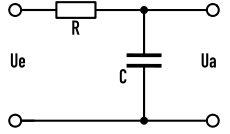
\includegraphics[height=6cm]{tiefpass.png}
  \caption{Einfacher Teifpass [1]}
  \label{abb1}
\end{figure}

%%\newpage

 \subsection{Schaltung als Umkehr-Integrator und -Differentiator}
Um die Funktionsweise des Operationsverstärkers als Umkehr-Integrator und Differentiator zu untersuchen, wurde die Ausgangsspannung $U_\text{A}$ in Abhängigkeit von der Frequenz gemessen. Die Eingangsspannung $U_1$ lag während der Messung durchgehend bei $U_1$=420 mV.
Die jeweils verwendeten Bauteile sind den Tabellen zu entnehmen.
%Beim Umkehr-Integrator und Differentiator wurden die selben Bauteile verwendet. Somit kam eine Kapazität mit $C$=1000 nF und ein Widerstand $R$=0,47 $\text{k}\Omega$ zum Einsatz.
In den Tabellen 6 und 7 sind die Messwerte aufgeführt und in den Abbildungen \ref{int} und \ref{dif} graphisch dargestellt. Dazu wurden die Verhältnisse $\frac{U_\text{A}}{U_1}$ wie bei Teilaufgabe a) geplottet.

Außerdem wurden beim Umkehr-Differentiator die Korrelationen der Messwerte (bis zum jeweiligen Messwert in der Tabelle) berechnet, da hier , im Gegensatz zum Umkehr-Integrator, nicht im gesamten Messbereich ein mit der Theorie verträglicher Verlauf vorliegt.
Wie zu erkennen ist, ist die Korrelation ab dem dreizehntem Messwertepaar, kleiner als 90\%, weshalb nur die vorherigen Werte für die lineare Ausgleichsrechnung benutzt werden.
\


\iffalse
 \begin{minipage}{0.6\textwidth}
\begin{tabular}{@{}l|r@{}}
 \multicolumn{2}{c}{Tabelle 6: Messwerte Umkehr- Integrator} \\

    \toprule
     \multicolumn{2}{c}{$C$=22 nF, $R$=0,47 k$\Omega$} \\
     \multicolumn{2}{c}{$U_1$=420 mV} \\
     \cmidrule(r){1-2}
    $\frac{\nu}{kHz}$ & $\frac{U_A}{V}$ \\
    \midrule
       0,1 & 23,9  \\
     0,25 & 19,1  \\
     0,5 & 10,1 \\
     0,75 & 7,0 \\
     1 & 4,8  \\
     1,25 & 4,1 \\
     1,5 & 3,5 \\
     1,75 & 2,9 \\
     2,0 & 2,7 \\
     2,25 & 2,21 \\
     2,75 & 1,85 \\
     3,0 & 1,69 \\
     3,25 & 1,57 \\
     3,5 & 1,49 \\
     3,75 & 1,37 \\
     4,0 & 1,29 \\
     4,25 & 1,25 \\
     4,5 & 1,17 \\
     4,75 & 1,13 \\
     5,0 & 1,01 \\
     5,25 & 0,94 \\
     5,5 & 0,90 \\
     5,75 & 0,86 \\
     6,0 & 0,84 \\
     			\\
     \bottomrule

\end{tabular}

\end{minipage}
\begin{minipage}{0.6\textwidth}
\begin{tabular}{@{}lr@{}lr@{}}
     \multicolumn{2}{c}{Tabelle 7: Messwerte Differentiator} \\
      \toprule
    \multicolumn{2}{c}{$C$=1000 nF, $R$=0,47 k$\Omega$} \\
     \multicolumn{2}{c}{$U_1$=420 mV} \\
    \cmidrule(r){1-2}
    $\frac{\nu}{Hz}$ & $\frac{U_A}{V}$ \\

    \midrule
	1	& 1,25 \\
	2	& 2,17 \\
	3	& 2,85 \\
    	4	& 3,22 \\
    	5	&  3,5 \\
    	6	& 3,7 \\
    	7	& 3,82 \\
    	8	& 3,9 \\
	9	& 3,98 \\
	10	& 4,2 \\
     	11	& 4,2 \\
     	12	& 4,3 \\
     	13	& 4,3 \\
     	14	& 4,3 \\
     	15	& 4,3 \\
     	16	& 4,3 \\
     	17	& 4,3 \\
     	18	& 4,3 \\
     	19	& 4,3 \\
     	20	& 4,3 \\
     	21	& 4,3 \\
     	22	& 4,3 \\
     	23	& 4,3 \\
     	24	& 4,3 \\
     	25	& 4,3 \\
     \bottomrule
\end{tabular}
\end{minipage}
\fi



\begin{table}
\centering
\begin{tabular}{p{2cm}|p{2cm}}

	$\frac{\nu}{\si{\kilo \hertz}}$ & $\frac{U_A}{\si{\volt}}$ \\

\toprule
0,1 & 23,9  \\
0,25 & 19,1  \\
0,5 & 10,1 \\
0,75 & 7,0 \\
1 & 4,8  \\
1,25 & 4,1 \\
1,5 & 3,5 \\
1,75 & 2,9 \\
2,0 & 2,7 \\
2,25 & 2,21 \\
2,75 & 1,85 \\
3,0 & 1,69 \\
3,25 & 1,57 \\
3,5 & 1,49 \\
3,75 & 1,37 \\
4,0 & 1,29 \\
4,25 & 1,25 \\
4,5 & 1,17 \\
4,75 & 1,13 \\
5,0 & 1,01 \\
5,25 & 0,94 \\
5,5 & 0,90 \\
5,75 & 0,86 \\
6,0 & 0,84 \\
%\midrule

%\multicolumn{2}{c}{$\overline{n}$} & \multicolumn{2}{c} {1,56 $\pm$ 0,02} \\
\bottomrule
\end{tabular}
\caption{Messwerte Integrator mit $C=\SI{22}{\nano \farad},R=\SI{0,47}{\kilo \ohm},U_1=\SI{420}{\milli \volt}$.}
\label{tab:int}
\end{table}


\begin{table}
\centering
\begin{tabular}{p{2cm}|p{2cm}|c}

$\frac{\nu}{\si{\kilo \hertz}}$ & $\frac{U_A}{\si{\volt}}$ & Korrelation \\

\toprule
1	& 1,25 & -\\
2	& 2,17 & 1\\
3	& 2,85 & 0,99\\
    4	& 3,22  & 0,98\\
    5	&  3,5 & 0,97\\
    6	& 3,7 & 0,96\\
    7	& 3,82 & 0.95\\
    8	& 3,9 & 0,93\\
9	& 3,98 & 0,92\\
10	& 4,2 & 0,92\\
    11	& 4,2 & 0,90\\
    12	& 4,3 & 0,90\\
    13	& 4,3 & 0,89\\
    14	& 4,3 & 0,88\\
    15	& 4,3 & 0,87\\
    16	& 4,3 & 0,86\\
    17	& 4,3 & 0,85\\
    18	& 4,3 & 0,83\\
    19	& 4,3 & 0,82\\
    20	& 4,3 & 0,81\\
    21	& 4,3 & 0,79\\
    22	& 4,3 & 0,78\\
    23	& 4,3 & 0,77\\
    24	& 4,3 & 0,76\\
    25	& 4,3 & 0,75\\
%\midrule

%\multicolumn{2}{c}{$\overline{n}$} & \multicolumn{2}{c} {1,56 $\pm$ 0,02} \\
\bottomrule
\end{tabular}
\caption{Messwerte Differentiator mit $C=\SI{1000}{\nano \farad},R=\SI{0,47}{\kilo \ohm},U_1=\SI{420}{\milli \volt}$.}
\label{tab:diff}
\end{table}

\newpage
\noindent
Die gefittetten Ergebnisse sind:
 \begin{align}
     f_{\text{int}}(\nu)&=(5,39\pm0,38)\cdot \left(\frac{\nu}{\text{Hz}}\right)^{0,26\pm0,02}\\
     f_{\text{diff}}(\nu)&=(11,82\pm0,13)\cdot \left(\frac{\nu}{\text{Hz}}\right)^{-0,97\pm0,01}
 \end{align}
 mit den Steigungen der Geraden im doppelt-logarithmischen Diagramm:
 \begin{align}
   m_1&=0,26\pm0,02\\
   m_2&=-0,97\pm0,01
 \end{align}
\begin{figure}[!h]
\centering
\includegraphics[width=0.7\textwidth]{differentiatorplot}
\caption{Umkehr-Differentiator}
\label{dif}
\end{figure}
\begin{figure}[!h]
\centering
\includegraphics[width=0.7\textwidth]{integratorplot}
\caption{Umkehr-Integrator}
\label{int}
\end{figure}
\newpage
\noindent
Im Folgenden ist das Ausgangssignal $U_A$ bei einer Sinus-, Dreieck-, oder Rechtecksspannung aufgenommen, um die Funktionsweise der beiden Schaltungen zu überprüfen.Bei dem Integrator wird das Eingangssignal integriert, erwartet wird also die Stammfunktion der Speisespannung $U_1$. Analog dazu wird beim Differentiator das Eingangssignal differentiert, erwartet wird also die Ableitung.
%Die $\frac{1}{\nu}$-Proportionalität für die Umkehr-Integrator-Schaltung und Differentiator-Schaltung besitzt Gültigkeit im gesamten Messbereich. Lediglich sind minimale Abweichungen beim Umkehr-Integrator-Schaltung zu beobachten. Außerdem wurde das Ausgangssignal bei einer Sinus-, Dreieck-, oder Rechtecksspannung aufgenommen, um die Funktionsweise der beiden Schaltungen zu überprüfen. Bei dem Integrator wird das Eingangssignal integriert, erwartet wird also die Stammfunktion. Analog dazu wird beim Differentiator das Eingangssignal integriert, erwartet wird also die Ableitung.
\begin{figure}[H]%H statt !h !!!!!!!!!!!, DANN MACHT ER ES AUCH HIER IM TEXT
\centering
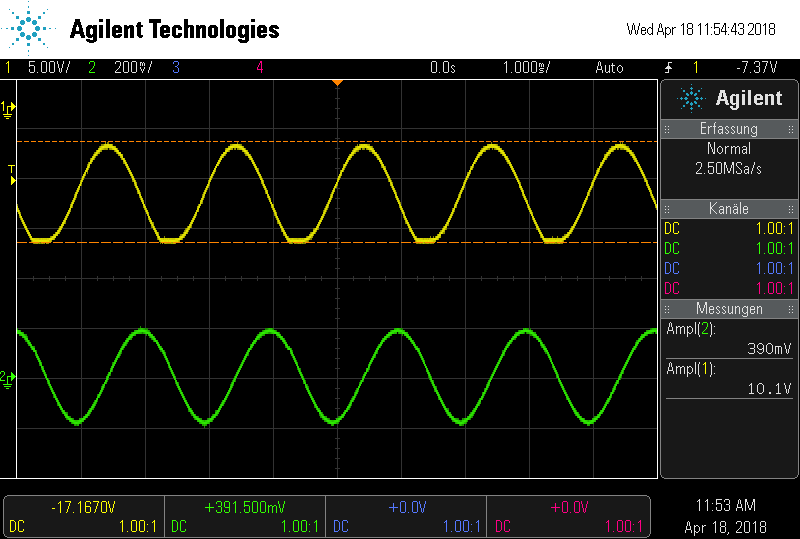
\includegraphics[width=0.4\textwidth]{aufnahmen_neu/scope_187.png}
\caption{Sinusspannung }
\label{verstaerker}

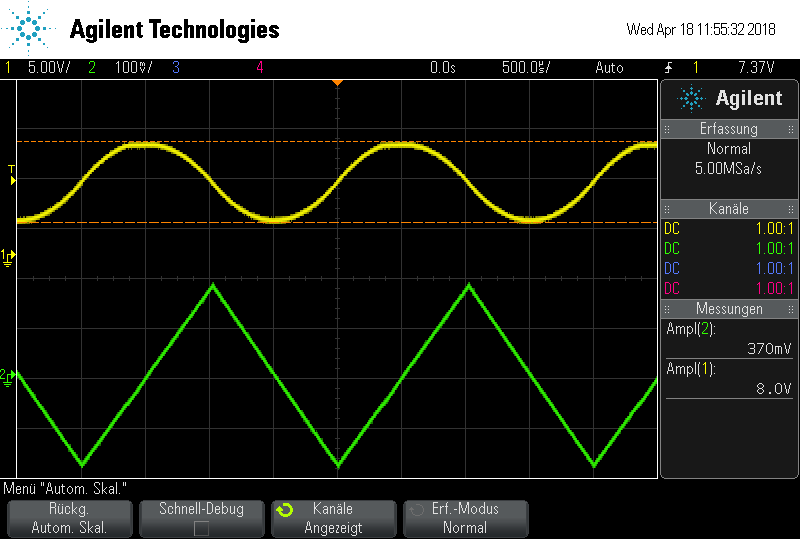
\includegraphics[width=0.4\textwidth]{aufnahmen_neu/scope_189.png}
\caption{Dreicksspannung}
\label{verstaerker}

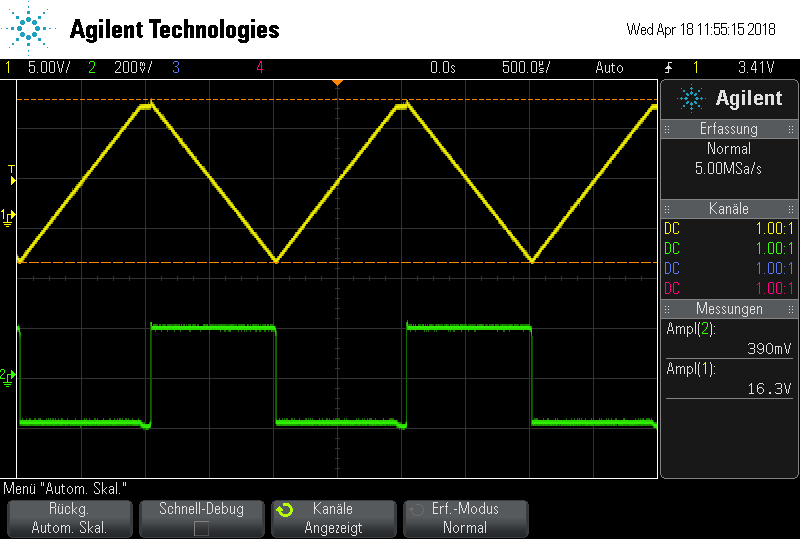
\includegraphics[width=0.4\textwidth]{aufnahmen_neu/scope_188.png}
\caption{Rechtecksspannung}
\label{verstaerker}

\end{figure}
%\\
%\noindent
In den Abbildungen 15 bis 17 sind die Bilder für den Integrator zu sehen.  Das grüne Singal ist das Eingangssignal und das gelbe Signal das Ausgangssignal.
Aus der Sinusspannung wird eine Kosinusspannung, aus der Dreieckspannung eine parabelförmige Spannung, aus der Rechteckspannung eine Dreieckspannung.
\begin{figure}[H]
\centering
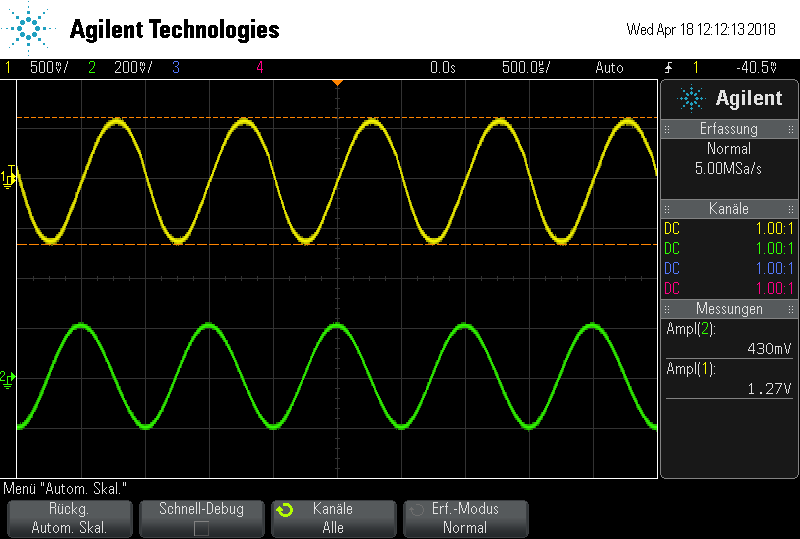
\includegraphics[width=0.4\textwidth]{aufnahmen_neu/scope_190.png}
\caption{Sinusspannung}
\label{verstaerker}

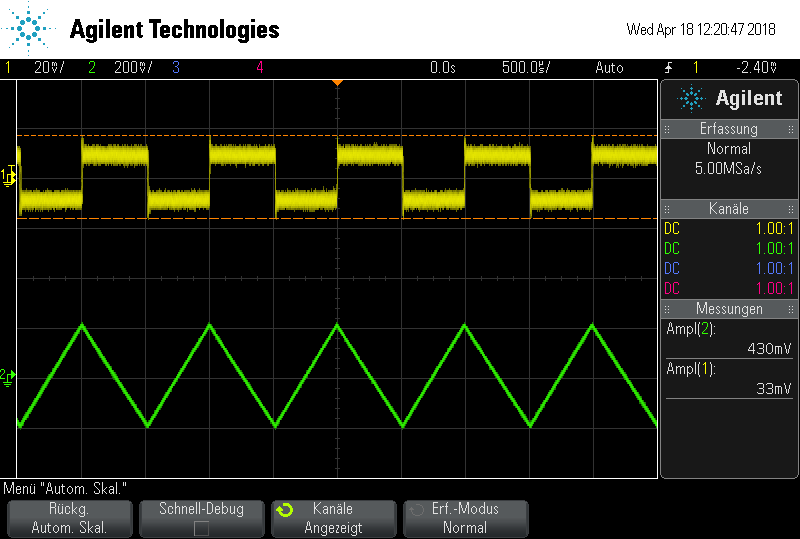
\includegraphics[width=0.4\textwidth]{aufnahmen_neu/scope_191.png}
\caption{Dreiecksspannung}
\label{verstaerker}

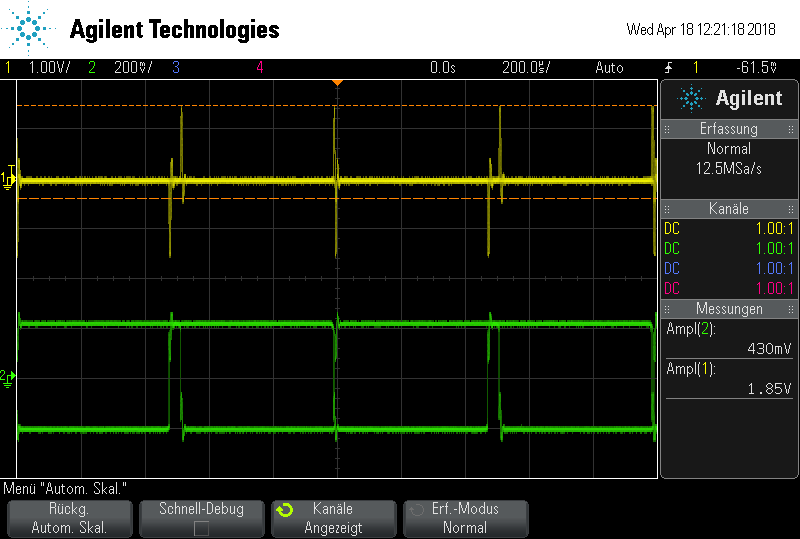
\includegraphics[width=0.4\textwidth]{aufnahmen_neu/scope_193.png}
\caption{Rechtecksspannung}
\label{verstaerker}
\end{figure}
%%%\newpage
\noindent
Analog ergibt sich beim Differentiator aus der Sinusspannung eine Kosinusspannung, aus der Dreieckspannung eine Rechteckspannung, und aus der Rechteckspannung wird eine periodische Spannung aus Delta-peaks.
\newpage
\subsection{Schmitt-Trigger als Schalter}
 Die beim Schmidt-Trigger verwendeten Widerstände, die Betriebsspannungsamplitude des Operationsverstärkers und die Spannungsamplitude der Ausgangspannung (welche ohne Verluste identisch zur Betriebsspannungsamplitude ist) sind:\\
 \\ \textbf{Messung 1}:
 \begin{align}
 R_1 &= \SI{0,47}{\kilo \ohm}\\
 R_\text{p} &= \SI{10,01}{\kilo \ohm}\\
 2U_B&=\SI{28,3}{\volt}\\
 2U_A&=\SI{26,5}{\volt}
 %U_\text{B+} &= 14{,}28 \,\text{V}\\
 %U_\text{B-} &= -14{,}25 \,\text{V}\\
 %\overline{U}_\text{B} &= (14{,}26\pm 0{,}01)\,\text{V}
 \end{align}
 Der theoretische Schwellenwert ergibt sich zu
 \begin{align}
 U_\text{schwell,th} = 665\,\text{mV}\;.
 \end{align}
 Experimentell wurde die Amplitude der Eingangsspannung an der Stelle, bei denen der Trigger umschaltet bestimmt:
 \begin{align}
 U_\text{schwell,exp} &= 700\,\text{mV}\;,\\
 \end{align}
 Ein Bild der Messung am Umschaltpunkt ist in Abbildung \ref{trigger1} zu sehen.
  \begin{figure}[!h]
\centering
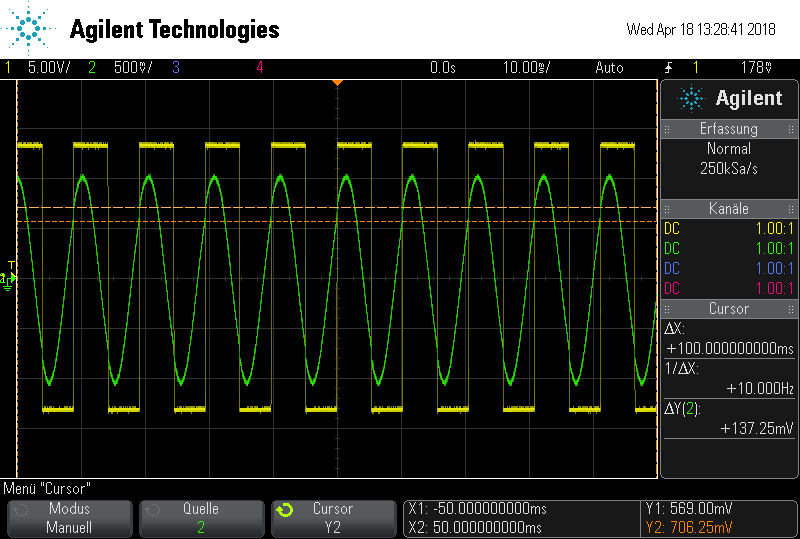
\includegraphics[width=0.6\textwidth]{aufnahmen_neu/scope_195.png}
\caption{Schmitt- Trigger}
\label{trigger1}
\end{figure}

\textbf{Messung 2}
\begin{align}
R_1 &= \SI{10,01}{\kilo \ohm}\\
R_\text{p} &= \SI{99,5}{\kilo \ohm}\\
2U_B&=\SI{28,3}{\volt}\\
2U_A&=\SI{26,7}{\volt}
%U_\text{B+} &= 14{,}28 \,\text{V}\\
%U_\text{B-} &= -14{,}25 \,\text{V}\\
%\overline{U}_\text{B} &= (14{,}26\pm 0{,}01)\,\text{V}
\end{align}
Der theoretische Schwellenwert ergibt sich zu
\begin{align}
U_\text{schwell,th} = \SI{1,42}{\volt}.
\end{align}
Experimentell wurde die Amplitude der Eingangsspannung an der Stelle, bei denen der Trigger umschaltet bestimmt:
\begin{align}
U_\text{schwell,exp} &= \SI{1,31}{\volt}\\
\end{align}
Ein Bild der Messung am Umschaltpunkt ist in Abbildung 21 zu sehen.
 \begin{figure}[!h]
\centering
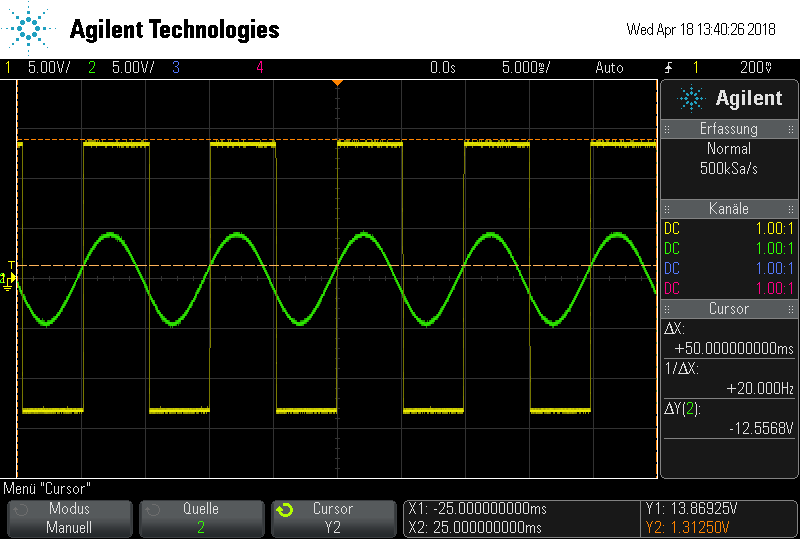
\includegraphics[width=0.6\textwidth]{aufnahmen_neu/scope_196.png}
\caption{Schmitt- Trigger}
\label{schmitttrigger}
\end{figure}

 \subsection{Gedämpfte Schwingung}
 Für den Aufbau der Schaltung von 2 Integratoren mit einem Umkehrverstärker nach Abbildung \ref{harm} wurden folgende Bauteile verwendet:
 \begin{align}
	 \begin{split}
	  R &= \SI{10}{\kilo \ohm}\\
	  R_1 &= \SI{1}{\kilo \ohm}\\
	  C &= \SI{24}{\nano \farad}
 %R_1 &= 9,96\,\text{k}\Omega\\
 %R_2 &= 9,97\,\text{k}\Omega\\
  %R_3 &= 0,99\,\text{k}\Omega\\
 %R_4 &= 0,99,\text{k}\Omega\\
  %R_5 &= 99,9\,\text{k}\Omega\\
 %C &= 100\,\text{nF}
   \end{split}
 \end{align}
 Die sehr geringen Abweichungen der Widerstände vom Wunschwert (Abbildung 6) können hier vernachlässigt werden.
 Für die ungedämpfte Schwingung wurde die Frequenz
 \begin{equation}
   \nu_{exp}=\SI{667,2}{Hz}
 \end{equation}
 notiert.
 Die aus $R$ und $C$ berechnete Theoriefrequenz ergibt sich zu:
 \begin{equation}
   \nu_{th}=\frac{1}{T_{th}}=\frac{1}{2 \pi RC} \approx \SI{663,15}{Hz}
 \end{equation}\\
 \\Die Amplitude der gedämpften Schwingung wird in Abhängigkeit von der Zeit, mit Hilfe eines Oszilloskops untersucht.
 Die an die Messwerte gefittete Theoriekurve ist
\begin{equation}
  U_{A,exp}(t)= U_0e^{\frac{t}{\tau_{exp}}}\text{sin}\left( \frac{2 \pi t}{T_{exp}}+\varphi \right)
%  \approx
%  3,31e^{\frac{t}{7,22}}\text{sin}\left(\frac{2 \pi t}{0,0014}+2,39\right)
\end{equation}
und die gefitteten Werte sind:
\begin{align}
  U_0 &= \SI{3,31 \pm 0,02}{\volt}\\
  \tau_{exp} &= \SI{7,22 \pm 0,03}{\milli \second}\\
  T_{exp} &= \SI{1,42 \pm 0,00}{\milli \second}\\
  %T_{exp} &= \SI{0,0014 \pm 0,0000}{\milli \second}\\
  \varphi &= 2,39 \pm 0,00
\end{align}
Die Messwerte sowie Fit sind in Abb. \ref{test1} dargestellt.
%  \begin{align}
%U_{Theorie}(t)=\alpha \cdot e^{\beta \cdot t} + \gamma
%=(75.61\pm 3,59) \cdot e^{(-0,82\pm 0,13) \cdot t} + (3.12\pm3.17)
 %\end{align}
 Der theoretisch zu erwartende Wert $\tau_{th}$ folgt aus dem Widerstand $R$ und der Kapazität $C$ mit $|\eta|$ =1 zu
\begin{align}
\tau _{th} = \SI{4,8}{\milli \second}. %ist neuer wert
 \end{align}
 \begin{figure}[!h]
\centering
\includegraphics[width=0.8\textwidth]{4.5/gedaempft.pdf}
\caption{Ausgleichsfunktion und Messwerte der gedämpften Schwingung}
\label{test1}
\end{figure}
\
\
\

\iffalse
\begin{center}
\begin{tabular}{@{}lr@{}}
\toprule
  t/ms & U/V \\
  \midrule
5,7 & 3.5766 \\
12,7 & 2.6344 \\
19,5 & 1.9673 \\
26.5 & 1.4661 \\
33,2 & 1.0754 \\
40,4 & 0.7814 \\
48,8 & 0.5917 \\
55,8 & 0.4952 \\
     			\\
     \bottomrule
\\
Tabelle 6: Spannungsverlauf in Abhängigkeit von der Zeit
\end{tabular}
\end{center}
\fi

%\begin{figure}[!h]
%\centering
%\includegraphics[width=0.8\textwidth]{4.5/gedaempft_daempfung.pdf}
%\caption{Dämpfung der gedämpften Schwingung}
%\label{test2}
%\end{figure}

\iffalse
\section{Diskussion}
\label{sec:Diskussion}
In diesem Teil wird über die Ergebnisse und mögliche Fehler, durch Messfehler und Messungenauigkeiten etc. diskutiert.
\begin{itemize}
\item Beim gegengekoppelten invertierenden Linearverstärker liefern die Ergebnisse für die vier unterschiedlichen Frequenzgänge folgende Ergebnisse: Bei der ersten Frequenzgangmessung kann man davon sprechen, dass die Verstärkung nahe des Teilerverhältnises $R_\text{N}/R_1$ liegt. Jedoch ist bei den zwei nächsten Messungen der unterschied viel größer. Zuletzt beim letzten Teil war keine vernünpftige Auswertung möglich da wir zwei fast gleiche Widerstände verbaut und somit einen $R_\text{N}/R_1= 1,01$ hatten. Demzufolge haben wir durchgehend gleiche Werte gemessen.
\item Unsere gemessenen Werte lieferten für den Differentiator keine brauchbaren Ergebisse, da wir bei der Messung die Bauteile miteinander kurzgeschlossen und somit die Messung verfälscht haben. Mit den Werten die wir anschließend bekommen haben, zeigte die Umkehr-Integrator-Schaltung und die Differentiator-Schaltung die erwartete Funktionalität.
\item Bei der Schaltung des Schmitt-Triggers stimmen die Werte $U_\text{schwell,th}$ und $U_\text{schwell,exp}$ mit einer Abweichung von$≈13,1\%$ prozent überein.
\item Bei der Messung der gedämpften harmonischen Schwingung haben wir für die gemessene Abklingdauer eine größe Abweichung von ca. $ 60\%$.
\end{itemize}
\fi


\section{Diskussion}
\label{sec:Diskussion}
In diesem Teil wird über die Ergebnisse und mögliche Fehler, durch Messfehler und Messungenauigkeiten etc. diskutiert.
\begin{itemize}
\item \textbf{4.2) Gegengekoppelter Linearverstärker:} Beim idealen Operationsverstärker entspricht die Verstärkung $V'$ dem Verhältniss $R_N/R_1$, da von einer unendlichgroßen Leerlaufverstärkung ausgegangen wird (siehe Formel \ref{lappen1}).
Der Vergleich der Verstärkung $V'$ des realen Operationsverstärkers mit diesem Verhältniss, zeigt also wie nah das reale Bauelement am idealen ist.
$V'$, $R_N$ und $R_N/R_1$ aller vier aufgenommenen Frequenzgänge (vier verschiedene Kombinationen der Gegenkopplung $R_N$ und $R_1$) sind in unterer Tabelle aufgelistet.
\begin{table}
\begin{center}
\caption{Frequenzganguntersuchung}
\begin{tabular}{ccccc}
\hline
 Parameter& Messung 1&Messung 2&Messung3&Messung 4\\
 \hline $R_N$ / k$\Omega$ & 99,5 & 99,5 & 99,5 & 33,2 \\
  $R_1$ / k$\Omega$ & 10,0 & 33,2 & 1,0 & 1,0 \\
  $\frac{R_N}{R_1}$ & 9,9 & 3,0 & 99,5 & 33,2 \\
  $\bar{V}'$ & 10,23 \pm0,03 & 2,98 \pm 0,00 & 57,02 \pm 0,38 & 33,27 \pm 0,23 \\
  %$\frac{\nu'_g}{kHz}$ & 48,2 & 95,8 & 16,4 & 23,9 \\
  %$\frac{\nu'_g \bar{V}'}{kHz}$ & 492,12 &  285,48  & 935,13 & 795,15\\
   \hline
\end{tabular}
\end{center}
\end{table}
 Bei den Messungen/Frequenzgängen 1, 2 und 4 zeigen die ermittelten Versärkungen sehr gute Übereinstimmung mit dem Verhältnis $R_N/R_1$, ledeglich bei Messung 3 liegt eine Abweichung von über $40 \%$ vor, weshalb es sinnvoll ist die Leerlaufverstärkung des realen Operationsverstrkers für diesen Frequenzgang (nach Formel \ref{lappen1}) abzuschätzen:
\begin{equation}
  V\approx133,56
\end{equation}
Da der Unterschied der beiden Widerstände bei dieser Messung maximal war ($R_N=\SI{99,5}{\kilo \ohm},R_1=\SI{1,0}{\kilo \ohm}$), könnte dies der Grund für die vergleichsweise hohe Abweichung sein.
Oder der Widerstand $R_N$ dieser Messung wurde fehlerhaft ausgemessen, was ein falsch berechnetes Verhältnis $R_N/R_1$ zu Folge hat.
Denn die Leerlaufverstärkung sollte konstant sein, da bei allen Messungen der selbe Operationsverstärker verwendet wurde.

Die experimentel ermittelten Bandbreiteprodukte $\nu'_g \bar{V}'$, welche ebenfalls identisch sein sollten, sind in Tabelle (3) nachzusehen.
Die Werte zeigen eine relativ gute Konstanz.
Vorallem im Rahmen des Messfehlerintervalls können die Werte fast gleich sein.
Das liegt auch daran, dass die Fehler der Bandbreiteprodukte besonders bei den ersten beiden Messungen vergleichsweise groß sind, da die Fehler der Grenzfrequenzen hier schon am größten waren.
\begin{table}
\begin{center}
\caption{Frequenzganguntersuchung}
\begin{tabular}{ccccc}
\hline
 Parameter& Messung 1&Messung 2&Messung3&Messung 4\\
 \hline $R_N$ / k$\Omega$ & 99,5 & 99,5 & 99,5 & 33,2 \\
  $R_1$ / k$\Omega$ & 10,0 & 33,2 & 1,0 & 1,0 \\
  %$\frac{R_N}{R_1}$ & 9,9 & 3,0 & 99,5 & 33,2 \\
  %$\bar{V}'$ & 10,21 & 2,98 & 57,02 & 33,27 \\
  $\frac{\nu'_g}{kHz}$ & 74,99 \pm 16,0 & 258,38 \pm 90,0 & 15,02 \pm 0,6 & 23,88 \pm 2,4 \\
  $\frac{\nu'_g \bar{V}'}{kHz}$ & 767,15 \pm 160,0 &  769,94 \pm 270  & 861,81 \pm 35,0 & 800,83 \pm 80,0 \\
   \hline
\end{tabular}
\end{center}
\end{table}

\newpage
%Maximal ist die Abweichung mit 935,13 und 285,48 zwischen Frequenzgang 3 und 2.
\item \textbf{4.4) Umkehrdifferentiator/-integrator:}
Beim Umkehr-Differentiator ist nach Formel (\ref{timbugtu}) ist im logarithmischen Diagramm ein linearer Verlauf der Ausgangspannung $U_A$ als Funktion der Speisefrequenz $\nu$ zu erwarten.
Die Steigung sollte dabei positiv sein.
Wie in Abb. (\ref{dif}) zu erkennen, ist der erwartete Verlauf nur im Anfangsbereich der Messung gegeben.
Die berechnete Korrelation zeigt, dass ab dem dreizehntem Messwert, also ab einer Speisespannungsfrequenz von $\nu=\SI{13}{\hertz}$, eine Abweichung von über 10\% vorliegt, was als obere Grenze gewählt wurde.
Das heißt der Umkehr Differentiator sollte nur für kleinere Frequenzen als linear Verstärker genutzt werden, weil es danach zu einer Sättigung kommt.
Im Diagramm (\ref{dif}) wird die, nicht aus der Theorie zu erwartende, Sättigung der Ausgangspannung $U_A$ nach diesem Messwert besonders deutlich.
%Nach den ersten 6 Messwerten kommt es zu einer Sättigung bei ca. $\SI{10.2}{\volt}$.
%Der Operationsverstärker sollte also nur im Anfangsbereich (bis ca.$\SI{10}{\volt}$) als Umkehr-Differentiator verwendet werden.

Beim Umkehr-Integrator hingegen ist über den gesamten Messbereich die aus der Theorie zu erwartende Proportionalität $U_A\propto \nu$ gegeben.

Das Signal für die angelegte Dreieck-/Rechteck-/ und Sinusspannung hat bei beiden Schaltungen die erwartete Form (Ableitung/Stammfunktion).
Das Bild der Rechteckspannung beim Umkehr-Integrator entspricht zwar zwei überlagerten Rechteckspannungen, die Delta-Peaks des Ausgangssignals sind dennoch deutlich sichtbar.
%Wie in Abb. \ref{differentiator} zu sehen, ist die $1/\nu$ Proportionalität beim Umkehr-Integrator vorallem im Anfangsbereich ($\nu<\SI{500}{Hz}$) der Messung nicht gegeben.
%Beim Umkehr-Differentiator hingegen ist über den gesamten Messbereich die aus der Theorie zu erwartende Proportionalität $U_A\propto \nu$ gegeben.
%Das Signal für die angelegte Dreieck-/Rechteck-/ und Sinusspannung hat bei beiden Schaltungen die erwartete Form (Ableitung/Stammfunktion).
%Das Bild der Rechteckspannung beim Umkehr-Differentiator entspricht zwar zwei überlagerten Rechteckspannungen, die Delta-Peaks des Ausgangssignals sind dennoch deutlich sichtbar.
\item \textbf{4.4) Schmitt-Trigger:} Bei der Schaltung des Schmitt-Triggers stimmen die Werte der ersten Messung $U_\text{schwell,th=\SI{665}{\milli \volt}}$ und $U_\text{schwell,exp}=\SI{700}{\milli \volt}$ mit einer Abweichung von ca. $≈5\%$ überein.
Für die zweite Messung berechnet sich mit $U_\text{schwell,th=\SI{1,42}{\volt}}$ und $U_\text{schwell,th=\SI{1,31}{\volt}}$ die Abweichung zu $8\%$.
Insgesamt liegt relativ gute Übereinstimmung vor.
In der Theorie liegt die Sättigungsspannung des Schmitt-Triggers exakt bei der positiven bzw. negativen Betriebsspannung $U_B$, dies ist wegen einem realen Operationsverstärker und Widerstandsverlusten in der Praxis nur in guter Näherung der Fall, wie in der Auswertung zu sehen.
Dies muss bei praktischen Anwendungen berücksichtigt werden.
\item \textbf{4.5) Gedämpfte/ungedämpfte harmonische Schwingung:} Aus der Theorie ist ein Wert von $\tau_{th}=\SI{4,8}{\milli \second}$ für die Abklingdauer zu erwarten.
Der experimentelle Wert von $\tau_{exp}=\SI{7,2}{\milli \second}$ zeigt allerdings eine große Abweichung von  ca. $ 50,4\%$ zum theoretisch berechneten.
Das liegt sehr wahrscheinlich an den Problemen mit dem Potentiometer beim Messen, was Auswirkung auf $\eta$ hat, wodurch sich der theoretisch berechnete Wert verfälscht, da hier von $\eta=+1$ für die Berechnung ausgegangen wird.

Bei der zu messenden Frequenz $\nu$ ungedämpften Schwingung liegen bessere Ergebnisse vor, der theoretisch zu erwartende Werte $\nu_{th}=\SI{663,15}{\hertz}$ stimmt nahezu mit dem experimentell am Oszilloskop abgelesenen Wert $\nu_{exp}=\SI{667,2}{\hertz}$ überein, was von einer guten Messung zeugt.
Ebenso bestätigt es den Verdacht, dass die Fehler bei der gedämpften Messung hauptsächlich durch ein falsches $\eta \neq 1$, also falsche Einstellung des Potentiometers zustande kamen, da ein anderes $\eta$ (neben dem nun dazugeschalteten Rechteckgenaratur) der Hauptunterschied zur Schaltung der ungedämpften Schwingung ist.



 %Wir haben für die gemessene Abklingdauer $\tau_{exp}$ eine größe Abweichung von ca. $ 50,4\%$ von der theorietisch berechneten.
%Das liegt sehr wahrscheinlich an den Problemen mit dem Potentiometer beim Messen, was Auswirkung auf $\eta$ hat, wodurch sich der theoretisch berechnete Wert verfälscht.
%Bei der ungedämpften Schwingung stimmen die zu messende Frequenz der Ausgangsspannung $U_A$ und die der angelegten Spannnung $U_1$ nahezu überein.
\end{itemize}


\section{Literatur}

[1] Skript zu Versuch V51, Physikalisches Fortgeschrittenen Paktikum TU Dortmund

\noindent
[2] https://www.elektronik-kompendium.de/sites/bau/0209241.htm


\section{Anhang}

\end{document}
